\documentclass{article}

\usepackage{fouriernc,eulervm}
\usepackage[T1]{fontenc}
\usepackage[english]{babel}
\usepackage{float}
\usepackage{xcolor}
\usepackage[fleqn]{amsmath}

% Set page size and margins
% Replace `letterpaper' with`a4paper' for UK/EU standard size
\usepackage[a4paper,top=2cm,bottom=2cm,left=3cm,right=3cm,marginparwidth=1.75cm]{geometry}


% Useful packages
\usepackage{graphicx}
\usepackage[colorlinks=true, allcolors=blue]{hyperref}

\title{Random Forest for yield prediction on German NUTS3 Regions}
\author{Vincent Dlugosch}

\begin{document}
\maketitle


\begin{abstract}
	This experiment uses a random forest machine learning model to predict yearly yield anomalies for winter wheat in NUTS3 regions of Germany. The model is trained on climate data, derived climate indices, and static regional parameters. We explore two feature selection variants and evaluate the model's performance using data from 2007 to 2021.
\end{abstract}
\section{Introduction}
We use a random forest machine learning model to predict the yearly yield anomalies for winter wheat for NUTS3 regions in Germany. Training data consists of climate data, derived values from climate data such as SPI (Standard Precipitation Index), GDD (Growing Degree Days), and monthly frost days among others. Additional static parameters such as the mean elevation of the region and climate parameters such as mean precipitation per region derived from historical climate data are also used.
\section{Data Used}
As data for model training, we use 3 types of data. The data is averaged over each German NUTS3 region masked by the area where winter wheat was grown in the year 2018.
\subsection{Historical Climate Data}
This data, containing the climate variables: precipitation (pr), solar radiation (rsds), relative humidity (hurs), maximum temperature (tasmax), minimum temperature (tasmin), daily average temperature (tas), and wind speed (sfcWind) is available as daily data from 2007 to 2023 in 1 km * 1 km resolution over Germany.
It is resampled to monthly means and, as described before, subsequently averaged over each region masked by areas where winter wheat is grown.
\subsection{Derived Data}
This data is derived from the climate data. It includes:
\begin{itemize}
	\item SPI (Standard Precipitation Index) indicating periods of prolonged drought or abundance of precipitation compared to the observed time frame.
	\item Frost Days: Monthly sum of days when temperature is below 0 °C.
	\item GDD (Growing Degree Days): Accumulated heat per month that the plant can absorb. The base temperature for the calculation is 10 °C and the maximum threshold 30 °C.
	\item Heat Stress Days: The amount of days a certain threshold temperature is reached in a month. The threshold is 30 °C.
\end{itemize}
This data is also averaged over the regions and winter wheat acreage.
\subsection{Static Data}
This data is static data mapped to each NUTS3 region without any temporal resolution. It includes elevation data, average temperature in the region over the observed period, and average precipitation for the region. It is also cropped by winter wheat acreage.
\subsection{Yield Data}
Yield data ranging from 1979 to 2021 is available. Tons per acre data is available for 397 NUTS3 regions in Germany for various crops. As the climate data currently only ranges from 2007 to 2023, yield data available before is not used. As the model is only optimized for winter wheat, yield data for that crop is extracted. The yield data is processed to obtain weighted percentage values of yield anomalies compared to the 5-year period previous to the most recent year for the observed year.
\section{Features}
A subset of features is used, split into two variants on how the features are arranged.
\subsection{Features used}
Following is a list of features used for both variants:
\begin{itemize}
	\item Elevation data per region
	\item Mean regional precipitation per region
	\item Mean regional frost days per region
	\item Monthly SPI values per region and year
	\item Monthly GDD values per region and year
	\item Monthly frost day values per region and year
	\item Monthly heat day values per region and year
	\item Monthly solar radiation values per region and year
	\item Monthly average temperature values per region and year
	\item Monthly relative humidity values per region and year
	\item Monthly wind speed values per region and year
\end{itemize}
\subsection{Feature variants}
There are two variants for feature selection and shape tested.
In the first variant, each year and NUTS3 combination is one sample where the static data is assigned to each sample. The monthly data is split into one feature for each month-value combination, be it derived or raw climate data. Considering we use 9 months of the year for our prediction, we gain 9 features for each variable such as SPI or monthly precipitation.
The second variant encodes the month as a feature, expanding the number of samples to a multiple of the number of months observed. Each sample is such a combination of year, month, and NUTS3 region, and the corresponding variables are each one feature.
This approach necessitates a downsampling step as we now yield yearly predictions for each month. For this downsampling, a second random forest is trained using the outputs of each month as features and the real yield or yield anomaly as target, resulting in annualized data.
\section{Methods}
\subsection{Random Forest}
The model is built using the "scikit-learn" python library's RandomForestRegressor.
\subsubsection{Node feature relationship}
Each node corresponds to one feature when building the tree. The algorithm takes a subset of features on each node and tries to find the best feature and corresponding threshold to make the split on. Different thresholds are tried. For classification problems such as binary classification problems, the goal is to maximize the information gain for each split.
For regression problems, the variance of the target variable is tried to be minimized by trying different combinations of features and thresholds. The lower the variance, the better the quality of the split.
\subsubsection{Bootstrapping}
Each decision tree in the random forest is constructed using a bootstrapped dataset. Meaning a new dataset is created of the same size as the original with the difference that samples from the original dataset can be either omitted or appear multiple times in the bootstrapped dataset.
\subsubsection{Aggregation}
The random forest makes a prediction on the input data using each tree in the forest. The result is then aggregated using the average of all results.
The combination of "Bootstrapping" and "Aggregation" is called Bagging.
\subsubsection{Split calculation}
\begin{alignat*}{2}
	 & Weighted MSE &  & = w_L \cdot MSE_L + w_R \cdot MSE_R                \\
	 & where:       &  &                                                    \\
	 & w_L          &  & = \frac{n_L}{n_{total}}                            \\
	 & w_R          &  & = \frac{n_R}{n_{total}}                            \\
	 & MSE_L        &  & = \frac{1}{n_L} \sum_{i \in L} (y_i - \bar{y}_L)^2 \\
	 & MSE_R        &  & = \frac{1}{n_R} \sum_{i \in R} (y_i - \bar{y}_R)^2 \\
	 & \bar{y}_L    &  & = \frac{1}{n_L} \sum_{i \in L} y_i                 \\
	 & \bar{y}_R    &  & = \frac{1}{n_R} \sum_{i \in R} y_i                 \\
	 & n_L          &  & = \text{Number of samples in the left split}       \\
	 & n_R          &  & = \text{Number of samples in the right split}      \\
	 & n_{total}    &  & = n_L + n_R
\end{alignat*}


\subsubsection{Example}
\textbf{Split decision on node one:}
\\
\textbf{Split between SPI -2 and -1}

$n_L = 1, \ n_R = 4, \ n_{total} = 5, \ w_L = \frac{1}{5} = 0.2, \ w_R = \frac{4}{5} = 0.8$

$\bar{y}_L = -2$

$\bar{y}_R = \frac{(-1 + 1 + 1.2 + 1.7)}{4} = 0.725$

$MSE_L = (-5 + 2)^2 = 9$

$MSE_R = (-1 - 0.725)^2 + (1 - 0.725)^2 + (10 - 0.725)^2 + (12 - 0.725)^2 = 3 + 0.075 + 86 + 127 = 216.1$

$Weighted MSE = w_L \cdot MSE_L + w_R \cdot MSE_R = 0.2 \cdot 9 + 0.8 \cdot 216.1 = 174.6$
\\
\textbf{Split between SPI -1 and 1}

$n_L = 2, \ n_R = 3, \ n_{total} = 5, \ w_L = \frac{2}{5} = 0.4, \ w_R = \frac{3}{5} = 0.6$

$\bar{y}_L = \frac{(-2 - 1)}{2} = -1.5$

$\bar{y}_R = \frac{(1 + 1.2 + 1.7)}{3} = 1.3$

$MSE_L = (-5 + 1.5)^2 + (2 + 1.5)^2 = 12.25 + 12.25 = 25$

$MSE_R = (3 - 1.3)^2 + (10 - 1.3)^2 + (12 - 1.3)^2 = 2.89 + 75.69 + 114.49 = 193.07$

$Weighted MSE = w_L \cdot MSE_L + w_R \cdot MSE_R = 0.4 \cdot 25 + 0.6 \cdot 193.07 = 125.842$
\\
\textbf{Split between SPI 1 and 1.2}

$n_L = 3, \ n_R = 2, \ n_{total} = 5, \ w_L = \frac{3}{5} = 0.6, \ w_R = \frac{2}{5} = 0.4$

$\bar{y}_L = \frac{(-2 - 1 + 1)}{3} = -1$

$\bar{y}_R = \frac{(1.2 + 1.7)}{2} = 1.45$

$MSE_L = (-5 + 1)^2 + (2 + 1)^2 + (3 + 1)^2 = 16 + 9 + 16 = 41$

$MSE_R = (10 - 1.45)^2 + (12 - 1.45)^2 = 73.1 + 111.3 = 184.4$

$Weighted MSE = w_L \cdot MSE_L + w_R \cdot MSE_R = 0.6 \cdot 41 + 0.4 \cdot 184.4 =$\colorbox{yellow}{$98.36$}
\\
\textbf{Split between SPI 1.2 and 1.7}

$n_L = 4, \ n_R = 1, \ n_{total} = 5, \ w_L = \frac{4}{5} = 0.8, \ w_R = \frac{1}{5} = 0.2$

$\bar{y}_L = \frac{(-1 - 2 + 1 + 1.2)}{4} = -0.2$

$\bar{y}_R = 1.7$

$MSE_L = (-5 + 0.2)^2 + (2 + 0.2)^2 + (3 + 0.2)^2 + (10 + 0.2)^2 = 23.04 + 4.84 + 10.24 + 104.04 = 142.16$

$MSE_R = (12 - 1.7)^2 = 106.09$

$Weighted MSE = w_L \cdot MSE_L + w_R \cdot MSE_R = 0.8 \cdot 142.16 + 0.2 \cdot 106.09 = 135.34$
\\
\textbf{Split decision on node two:}
\\
\textbf{Split between SPI -2 and -1}

$n_L = 1, \ n_R = 2, \ n_{total} = 3, \ w_L = \frac{1}{3} = 0.33, \ w_R = \frac{2}{3} = 0.66$

$\bar{y}_L = -2$

$\bar{y}_R = 0$

$MSE_L = (-5 + 2)^2 = 9$

$MSE_R = 2^2 + 3^2 = 4 + 9 = 13$

$Weighted MSE = w_L \cdot MSE_L + w_R \cdot MSE_R = 0.33 \cdot 9 + 0.66 \cdot 13 =$\colorbox{yellow}{$11.58$}
\noindent
\\
\textbf{Split between SPI -1 and 1 }

$n_L = 2, \ n_R = 1, \ n_{total} = 3, \ w_L = \frac{2}{3} = 0.66, \ w_R = \frac{1}{3} = 0.33$

$\bar{y}_L = -1.5$

$\bar{y}_R = 1$

$MSE_L = (-5 + 1.5)^2 + (2 + 1.5)^2 = 12.25 + 12.25 = 25$

$MSE_R = (3 - 1)^2 = 4$

$Weighted MSE = w_L \cdot MSE_L + w_R \cdot MSE_R = 0.66 \cdot 25 + 0.33 \cdot 4 = 17.99$

\begin{figure}[H]
	\centering
	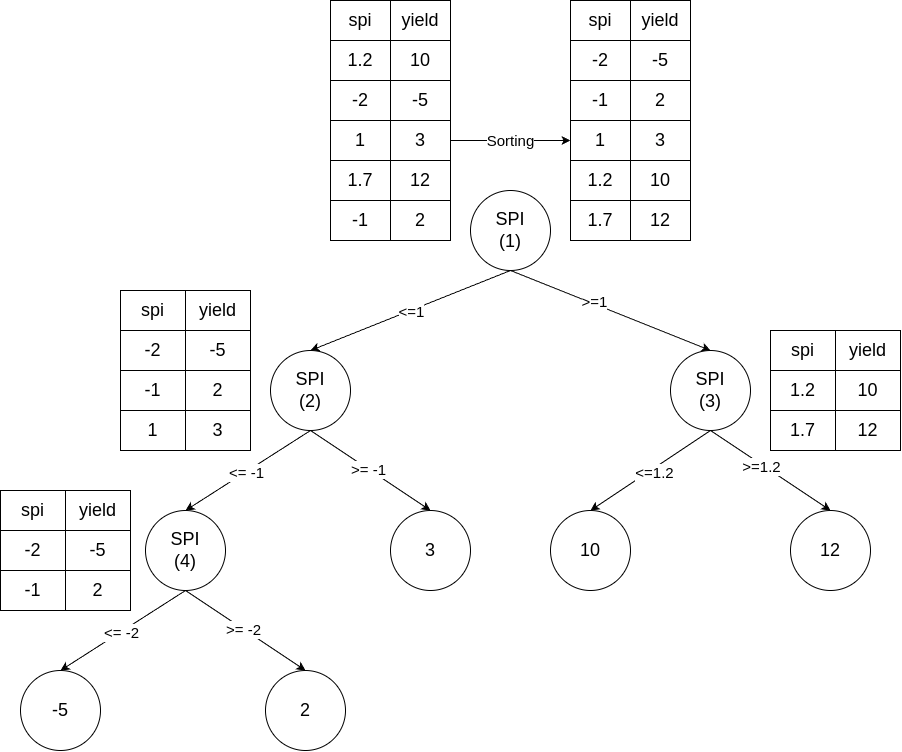
\includegraphics[width=1.0\textwidth]{./plots/DecisionTreeSplit.png}
	\caption{\label{fig:decision_tree_split}This Diagram illustrates how split decisions are taken in a decision tree.}
\end{figure}
\noindent
\subsubsection{Tree Parameters}
The random forest for both variants has a number of trees of 1000 the rest of the parameters are left at default.
The number of trees is chosen as the model performance does not degrade when adding more trees and no significant performance gains are observed after around 200 trees (Figure \ref{fig:n_trees_vs_performance}). Choosing 1000 trees gives headroom where the number of trees is not a performance constraint while still maintaining an acceptable speed of calculation for each random forest.
Further hyperparameter optimization is outstanding.
\begin{figure}[H]
	\centering
	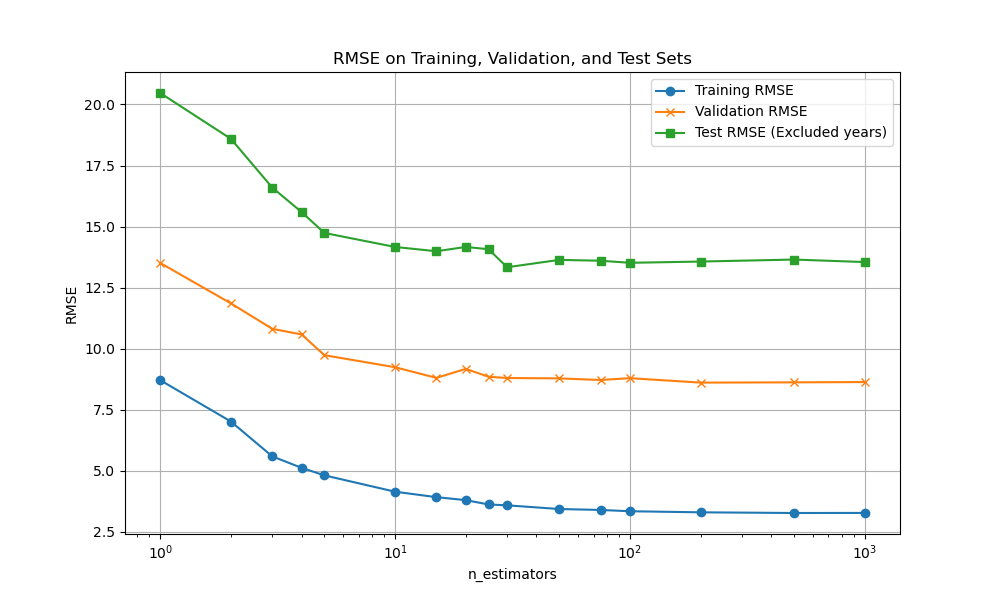
\includegraphics[width=1.0\textwidth]{../plots/model_performance_based_on_tree_count.png}
	\caption{\label{fig:n_trees_vs_performance}This graph shows model performance based on the number of trees used.}
\end{figure}
\subsection{Data Handling}
For training and evaluating the model's performance, different sets of data are used.
\subsubsection{Training Data}
Training data is the data the model uses to construct its trees. It contains both the features and corresponding targets.
For this model, training data comprises a random selection of 90\% of the available data ranging from 2007 to 2021, excluding the years 2015, 2020, and 2021.
\subsubsection{Validation Data}
Validation data is used to assess the model's performance during hyperparameter optimization.
In this case, a random selection of 10\% of the available data ranging from 2007 to 2021, excluding the years 2015, 2020, and 2021, is used.
As we are dealing with time series data, a random selection to validate on brings the risk of contaminating the training data with information of the current year, and the model might perform better on this subset than on real data.
\subsubsection{Test Data}
To mitigate that risk, whole yearly time series are excluded from both the training and validation data. Namely, the years 2015, 2020, and 2021. This selection is more or less arbitrary.
The model is applied to the test data in the end to assess the model's real-world performance.
\section{Results}
Both model variations perform well on the validation data.
\subsection{Features encoded as month value combination (variant 1)}
\subsubsection{Performance}
We can observe that the model predicts fairly well on the validation data with an R2 value of 0.71. While failing to predict on entirely unknown time series with an R2 value of only 0.12.
On the training data the model is able to predict with an R2 value of 0.96 suggesting overfitting.
As can be seen in table \ref{table:errors_on_datasets_variant_1} and \ref{table:errors_on_datasets_years_variant_1}.
\begin{table}[H]
	\centering
	\begin{tabular}{lcccc}
		\hline
		Data Split                        & MSE    & RMSE  & MAE   & R$^2$ \\
		\hline
		Training Data                     & 10.20  & 3.19  & 2.48  & 0.96  \\
		Validation Data                   & 74.39  & 8.62  & 6.62  & 0.71  \\
		Test (Excluded: 2015, 2020, 2021) & 181.04 & 13.46 & 10.68 & 0.12  \\
		\hline
	\end{tabular}
	\caption{\label{table:errors_on_datasets_variant_1} Random Forest performance metrics fo r training, validation, and test sets. The test set excludes data from years 2015, 2020, and 2021.}
\end{table}
\begin{table}[H]
	\centering
	\begin{tabular}{lcccc}
		\hline
		Excluded Year & MSE    & RMSE  & MAE   & R$^2$ \\
		\hline
		2015          & 210.24 & 14.50 & 11.41 & -0.28 \\
		2020          & 168.93 & 13.00 & 10.02 & 0.31  \\
		2021          & 163.89 & 12.80 & 10.61 & 0.19  \\
		\hline
	\end{tabular}
	\caption{\label{table:errors_on_datasets_years_variant_1} Random Forest performance metrics for test sets with individual years excluded.}
\end{table}
\begin{figure}[H]
	\centering
	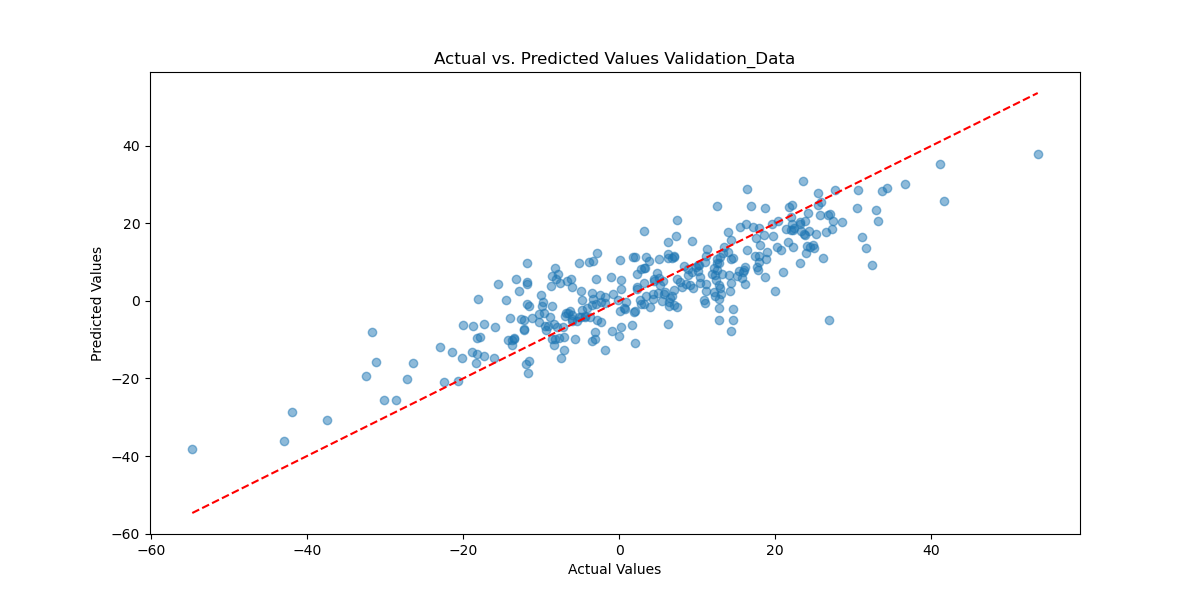
\includegraphics[width=1.0\textwidth]{./plots/scatter_Validation_Data.png}
	\caption{\label{fig:month_value_combination_scatter_validation_data}This scatter plot shows the relationship between prediction and actual values for the validation data.}
\end{figure}

\begin{figure}[H]
	\centering
	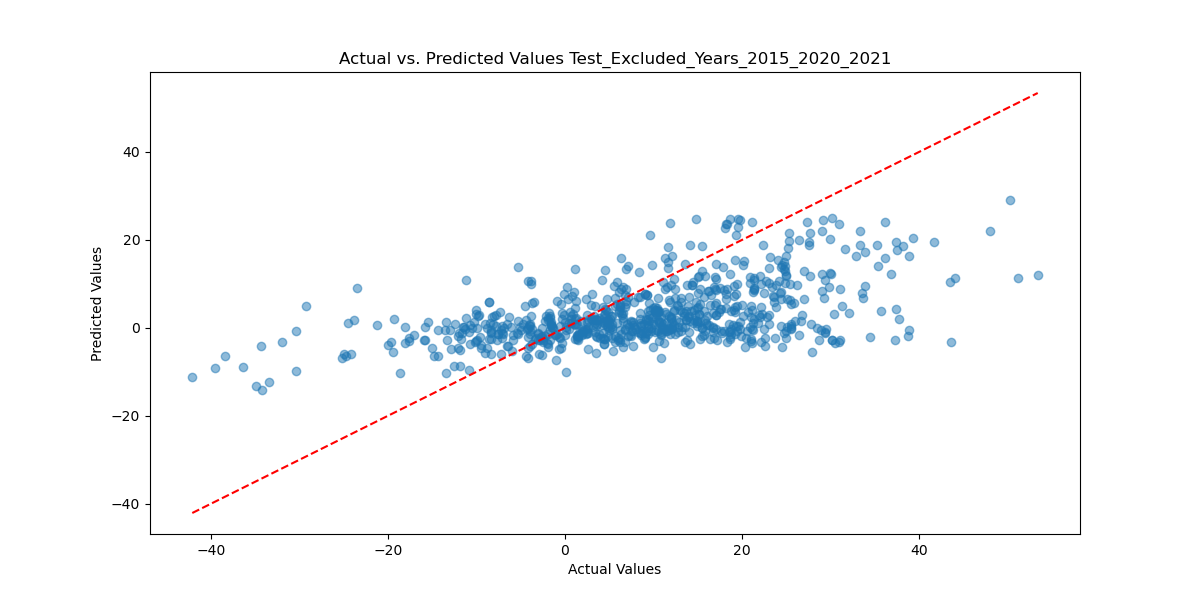
\includegraphics[width=1.0\textwidth]{./plots/scatter_Test_Excluded_Years_2015_2020_2021.png}
	\caption{\label{fig:month_value_combination_scatter_excluded_years}This scatter plot shows the relationship between prediction and actual values for the excluded years.}
\end{figure}

\subsubsection{Feature importance}
We get feature importance values for each Feature here the 15 most important features are shown (Table \ref{table:feature_importance_variant_1}).
\begin{table}[H]
	\centering
	\begin{tabular}{lc}
		\hline
		Feature                     & Importance \\
		\hline
		mean\_regional\_frost\_days & 0.133439   \\
		spi\_month\_10              & 0.061152   \\
		rsds\_month\_9              & 0.039532   \\
		frost\_days\_month\_10      & 0.038078   \\
		elevation                   & 0.035574   \\
		exceedance\_days\_month\_5  & 0.035009   \\
		hurs\_month\_4              & 0.029597   \\
		tas\_month\_11              & 0.025600   \\
		hurs\_month\_6              & 0.020628   \\
		tas\_month\_6               & 0.020308   \\
		rsds\_month\_6              & 0.018513   \\
		mean\_regional\_pr          & 0.018317   \\
		rsds\_month\_1              & 0.015174   \\
		hurs\_month\_5              & 0.014365   \\
		spi\_month\_12              & 0.014230   \\
		\hline
	\end{tabular}
	\caption{\label{table:feature_importance_variant_1} Feature importance for variant one.}
\end{table}
\subsection{Month as feature (variant 2)}
\subsubsection{Performance}
We can observe that the model still predicts fairly well on the validation data with an R2 value of 0.57. While improving its prediction for an unknown time series with an R2 value of 0.24 after month combination.
On the training data the model is able to predict with an R2 value of 0.94 suggesting overfitting.
\begin{table}[H]
	\centering
	\begin{tabular}{lcccc}
		\hline
		Data Split                                        & MSE    & RMSE  & MAE  & R$^2$ \\
		\hline
		Training Data                                     & 14.11  & 3.76  & 3.00 & 0.94  \\
		Validation Data                                   & 102.05 & 10.10 & 8.01 & 0.57  \\
		Test (Excluded: 2015, 2020, 2021)                 & 160.65 & 12.67 & 9.91 & 0.22  \\
		Test (Month Combiner, Excluded: 2015, 2020, 2021) & 156.73 & 12.52 & 9.79 & 0.24  \\
		\hline
	\end{tabular}
	\caption{Random Forest performance metrics for training, validation, and test sets. The test sets exclude data from years 2015, 2020, and 2021. The "Month Combiner" refers to a different data processing approach.}
\end{table}
\begin{table}[H]
	\centering
	\begin{tabular}{lcccc}
		\hline
		Excluded Year & MSE    & RMSE  & MAE   & R$^2$ \\
		\hline
		2015          & 217.86 & 14.76 & 11.79 & -0.34 \\
		2020          & 129.89 & 11.40 & 8.80  & 0.46  \\
		2021          & 134.21 & 11.59 & 9.14  & 0.35  \\
		\hline
	\end{tabular}
	\caption{Random Forest performance metrics for test sets with individual years excluded.}
\end{table}
\begin{figure}[H]
	\centering
	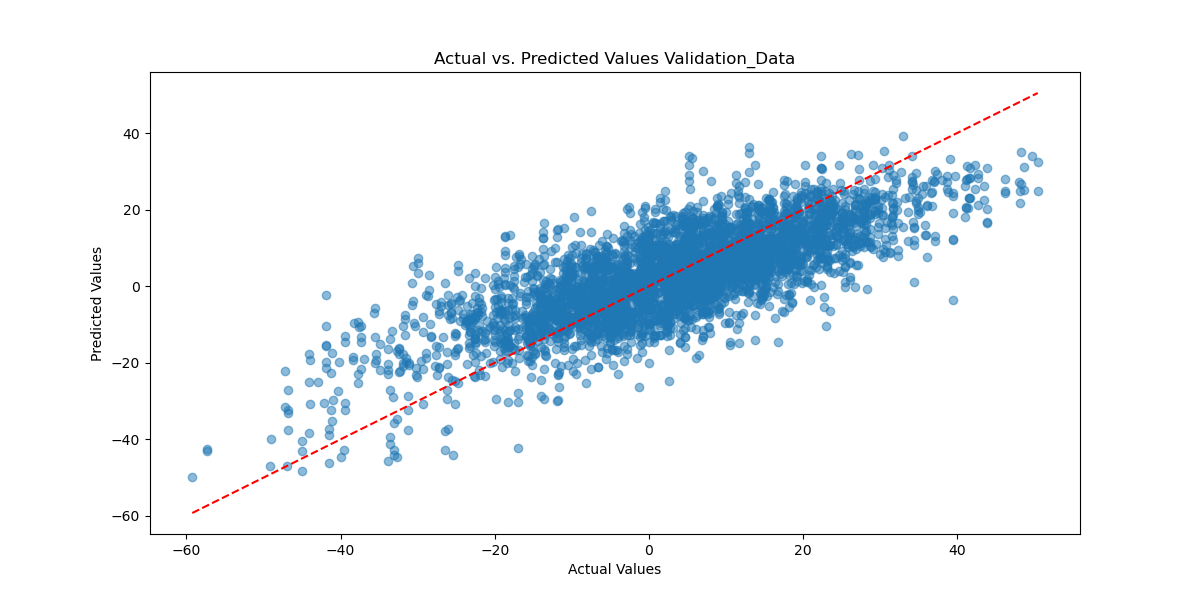
\includegraphics[width=1.0\textwidth]{./plots/scatter_Validation_Data_monthly.png}
	\caption{\label{fig:month_value_combination_scatter_validation_data_monthly}This scatter plot shows the relationship between prediction and actual values for the validation data.}
\end{figure}

\begin{figure}[H]
	\centering
	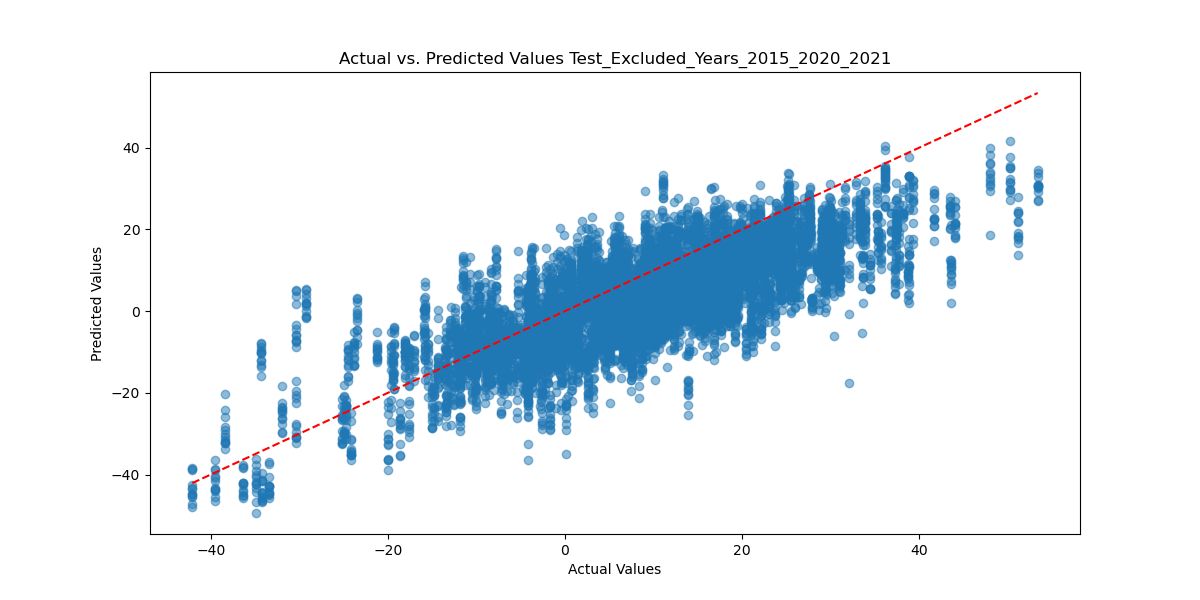
\includegraphics[width=1.0\textwidth]{./plots/scatter_Test_Excluded_Years_2015_2020_2021_monthly.png}
	\caption{\label{fig:month_value_combination_scatter_excluded_years_monthly}This scatter plot shows the relationship between prediction and actual values for the excluded years for monthly prediction before second model application.}
\end{figure}

\begin{figure}[H]
	\centering
	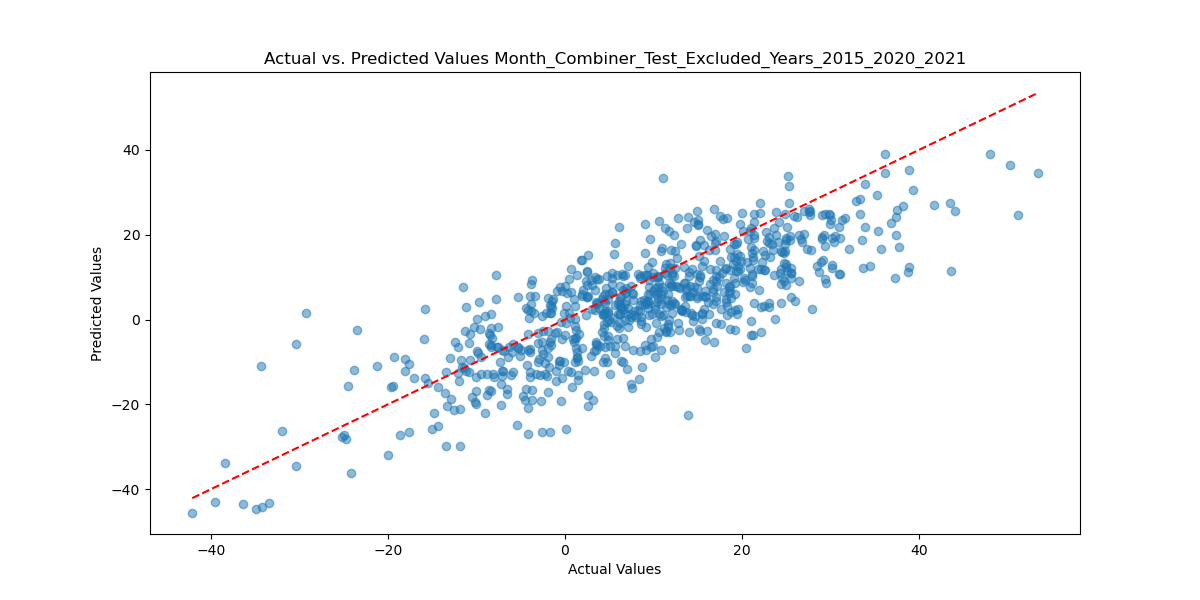
\includegraphics[width=1.0\textwidth]{./plots/scatter_Month_Combiner_Test_Excluded_Years_2015_2020_2021.png}
	\caption{\label{fig:combined_month_output_scatter_excluded_years}This scatter plot shows the relationship between prediction and actual values for the excluded years after second model application.}
\end{figure}

\subsubsection{Feature importance}
We get feature importance values for each Feature here the importance of all features are shown (Table \ref{table:feature_importance_variant_2}).
\begin{table}[H]
	\centering
	\begin{tabular}{lc}
		\hline
		Feature                     & Importance \\
		\hline
		mean\_regional\_frost\_days & 0.304568   \\
		elevation                   & 0.151538   \\
		mean\_regional\_pr          & 0.107865   \\
		spi                         & 0.085249   \\
		sfcWind                     & 0.079568   \\
		hurs                        & 0.077672   \\
		rsds                        & 0.058717   \\
		tas                         & 0.045216   \\
		frost\_days                 & 0.036800   \\
		gdd                         & 0.036471   \\
		exceedance\_days            & 0.016335   \\
		\hline
	\end{tabular}
	\caption{\label{table:feature_importance_variant_2} Feature importance for variant two.}
\end{table}
Feature importance for the month combining tree suggests the importance of each month in for the prediction (Table \ref{table:feature_importance_months_variant_2}).
\begin{table}[H]
	\centering
	\begin{tabular}{lc}
		\hline
		Month     & importance \\
		\hline
		October   & 0.443719   \\
		December  & 0.174008   \\
		June      & 0.155502   \\
		July      & 0.088585   \\
		February  & 0.036694   \\
		September & 0.027657   \\
		May       & 0.023309   \\
		April     & 0.016641   \\
		November  & 0.010131   \\
		August    & 0.009064   \\
		January   & 0.008154   \\
		March     & 0.006536   \\
		\hline
	\end{tabular}
	\caption{\label{table:feature_importance_months_variant_2} Feature importance of months for variant two.}
\end{table}
\pagebreak
\subsection{Including regional yield data in variant 1}
When including mean regional yield data in the feature set we can observe a significant jump in performance.
The regional mean is calculated such that the excluded years are not included in the calculation to prevent data contamination.
\subsubsection{Performance}
\begin{table}[H]
	\centering
	\begin{tabular}{lcccc}
		\hline
		Data Split                        & MSE    & RMSE  & MAE  & R$^2$ \\
		\hline
		Training Data                     & 5.50   & 2.34  & 1.79 & 0.98  \\
		Validation Data                   & 39.97  & 6.32  & 4.69 & 0.82  \\
		Test (Excluded: 2015, 2020, 2021) & 127.31 & 11.28 & 8.97 & 0.38  \\
		\hline
	\end{tabular}
	\caption{Random Forest performance metrics for training, validation, and test sets. The test set excludes data from years 2015, 2020, and 2021. Regional yield data included in features}
\end{table}

\begin{table}[H]
	\centering
	\begin{tabular}{lcccc}
		\hline
		Excluded Year & MSE    & RMSE  & MAE  & R$^2$ \\
		\hline
		2015          & 145.80 & 12.07 & 9.90 & 0.11  \\
		2020          & 101.94 & 10.10 & 7.72 & 0.59  \\
		2021          & 134.20 & 11.58 & 9.30 & 0.34  \\
		\hline
	\end{tabular}
	\caption{Random Forest performance metrics for test sets with individual years excluded. Regional yield data included in features}
\end{table}
\subsubsection{Feature Importance}
\begin{table}[H]
	\centering
	\begin{tabular}{lc}
		\hline
		Feature                   & Importance \\
		\hline
		mean\_regional\_ww\_yield & 0.5404     \\
		spi\_month\_10            & 0.0809     \\
		rsds\_month\_9            & 0.0265     \\
		frost\_days\_month\_10    & 0.0173     \\
		hurs\_month\_4            & 0.0116     \\
		rsds\_month\_4            & 0.0112     \\
		rsds\_month\_6            & 0.0111     \\
		hurs\_month\_10           & 0.0108     \\
		tas\_month\_11            & 0.0097     \\
		rsds\_month\_10           & 0.0085     \\
		rsds\_month\_5            & 0.0084     \\
		hurs\_month\_6            & 0.0075     \\
		tas\_month\_2             & 0.0074     \\
		frost\_days\_month\_12    & 0.0072     \\
		spi\_month\_6             & 0.0072     \\
		\hline
	\end{tabular}
	\caption{Top 15 most important features in the Random Forest model including mean regional yield.}
\end{table}
\end{document}
